\section{CÔNG NGHỆ ẢO HÓA CỦA ORACLE CLOUD}
\subsection{Khái niệm về ảo hóa}
Ảo hóa (Virtualization) là một công nghệ tiên tiến cho phép tạo ra các phiên bản ảo của tài nguyên phần cứng hoặc phần mềm, chẳng hạn như máy chủ, bộ nhớ, thiết bị lưu trữ, hệ điều hành hay mạng máy tính. Thay vì phải triển khai nhiều thiết bị vật lý tách biệt, ảo hóa sử dụng phần mềm trung gian (thường gọi là hypervisor) để mô phỏng và quản lý các chức năng phần cứng, từ đó cho phép nhiều máy ảo (Virtual Machine – VM) hoạt động song song trên cùng một máy chủ vật lý.

Trong môi trường ảo hóa, mỗi máy ảo hoạt động độc lập như một hệ thống riêng biệt, có hệ điều hành, ứng dụng và tài nguyên được phân bổ riêng. Điều này mang lại sự linh hoạt và hiệu quả cao trong việc sử dụng tài nguyên. Thay vì để một máy chủ vật lý chỉ chạy một ứng dụng và gây lãng phí tài nguyên, công nghệ ảo hóa giúp hợp nhất nhiều ứng dụng, dịch vụ trên cùng một hạ tầng phần cứng mà vẫn đảm bảo tính bảo mật, ổn định và hiệu năng.

Đối với doanh nghiệp, ảo hóa mang lại nhiều lợi ích to lớn: tối ưu hóa chi phí đầu tư phần cứng, giảm chi phí vận hành và bảo trì, tăng khả năng mở rộng, đồng thời nâng cao hiệu quả quản lý hệ thống công nghệ thông tin. Ngoài ra, công nghệ này cũng đóng vai trò nền tảng cho điện toán đám mây (Cloud Computing), cho phép triển khai các dịch vụ lưu trữ, điện toán, phân tích dữ liệu và ứng dụng doanh nghiệp trên quy mô lớn một cách linh hoạt.

Nhờ ảo hóa, các tổ chức có thể dễ dàng sao lưu, khôi phục dữ liệu, tạo môi trường kiểm thử – phát triển phần mềm an toàn mà không ảnh hưởng đến hệ thống chính, cũng như triển khai hạ tầng công nghệ thông tin theo mô hình dịch vụ (IT as a Service – ITaaS). Có thể nói, ảo hóa không chỉ giúp tận dụng tối đa sức mạnh của phần cứng mà còn góp phần thay đổi cách các doanh nghiệp xây dựng và vận hành hạ tầng số trong thời đại công nghệ 4.0.

\subsection{Một số kiến trúc ảo hóa}
\subsubsection{Hosted-based Virtualization (Ảo hóa dựa trên hệ điều hành nền tảng)}
 Đây là kiến trúc ảo hóa trong đó hypervisor (phần mềm ảo hóa) được cài đặt trên hệ điều hành chính (host OS). Điều đó có nghĩa là máy chủ phải cài đặt hệ điều hành trước, sau đó mới cài đặt hypervisor để tạo và quản lý các máy ảo (VM).

\begin{figure}[H] % cần gói float nếu muốn fix vị trí
    \centering
    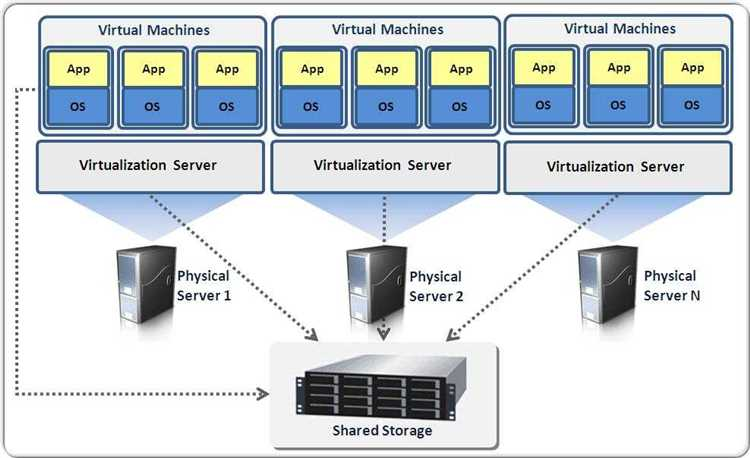
\includegraphics[width=0.9\textwidth]{Oracle_cloud/Hosted-based-Virtualization.jpg}
    \caption{Hosted-based Virtualization}
    \label{fig:cloud_intro}
\end{figure}

\begin{myitem}
\item Ưu điểm:
  \begin{mysubitem}
  \item Cài đặt và triển khai dễ dàng, thân thiện với người dùng.
  
  \item Phù hợp cho môi trường thử nghiệm, phát triển ứng dụng hoặc máy tính cá nhân.
  
  \item Có thể chạy nhiều hệ điều hành khác nhau trên cùng một máy.
  
  \end{mysubitem}

\item Nhược điểm:

  \begin{mysubitem}
  \item Hiệu năng thấp hơn vì hypervisor phải phụ thuộc và hoạt động gián tiếp thông qua hệ điều hành nền tảng.
  
  \item Ít phù hợp cho môi trường doanh nghiệp lớn hoặc hệ thống yêu cầu hiệu suất cao.

  \end{mysubitem}

\item Ví dụ: VMware Workstation, Oracle VirtualBox, Microsoft Virtual PC.
\end{myitem}

\subsection{Công nghệ ảo hóa máy chủ của Oracle cloud}
Oracle VM Server là một giải pháp ảo hóa máy chủ được Oracle phát triển, dựa trên nền tảng Xen Hypervisor nhưng đã được cải tiến và tích hợp chặt chẽ với Linux kernel nhằm tối ưu hóa hiệu suất và khả năng quản lý. Đây là một trong những sản phẩm chủ lực trong hệ sinh thái Oracle Virtualization, hỗ trợ triển khai các ứng dụng và dịch vụ doanh nghiệp trên hạ tầng ảo hóa mạnh mẽ, ổn định.

\begin{figure}[H] % cần gói float nếu muốn fix vị trí
    \centering
    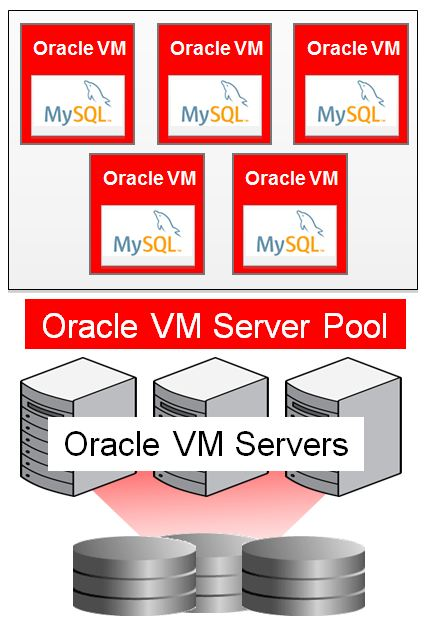
\includegraphics[width=0.65\textwidth]{Oracle_cloud/Oracle_VM_Server.jpg}
    \caption{Oracle VM Server}
    \label{fig:cloud_intro}
\end{figure}

Đặc điểm nổi bật:

\begin{myitem}
\item Dựa trên Xen Hypervisor nâng cao: Oracle VM Server sử dụng Xen – một công nghệ ảo hóa mã nguồn mở phổ biến, nhưng được Oracle tùy biến để đạt hiệu năng và độ ổn định cao hơn.


\item Hỗ trợ phần cứng và phần mềm phong phú: Có thể hoạt động với nhiều loại thiết bị, hệ thống file khác nhau, đồng thời tích hợp với phần mềm quản lý RAID để tăng cường khả năng bảo vệ dữ liệu.


\item Trình ảo hóa nhẹ và bảo mật: Hypervisor trong Oracle VM Server là thực thể duy nhất có đặc quyền cao nhất trong hệ thống, chiếm dung lượng rất nhỏ, giúp giảm thiểu nguy cơ tấn công và tối ưu tài nguyên.


\item Quản lý tài nguyên cơ bản: Oracle VM Server trực tiếp quản lý các thành phần quan trọng của hệ thống như CPU, bộ nhớ, quyền đặc biệt (privileges), và xử lý ngắt phần cứng (hardware interrupts).


\item Khả năng trừu tượng hóa cao: Thay vì chỉ gắn liền với phần cứng cụ thể, Oracle VM Server cung cấp lớp trừu tượng cho phép thực hiện cùng một tác vụ logic trên nhiều loại máy chủ vật lý khác nhau. Điều này mang lại sự linh hoạt trong triển khai và di chuyển khối lượng công việc.
\end{myitem}

Lợi ích khi sử dụng
\begin{myitem}
\item Hiệu năng cao: Nhờ quản lý trực tiếp tài nguyên phần cứng mà không cần thông qua hệ điều hành trung gian.

\item Khả năng mở rộng: Hỗ trợ triển khai trên nhiều máy chủ vật lý, dễ dàng mở rộng hệ thống khi nhu cầu tăng.


\item Tích hợp sâu với hệ sinh thái Oracle: Đặc biệt tối ưu cho cơ sở dữ liệu Oracle, Middleware, và các ứng dụng doanh nghiệp khác.


\item Bảo mật và ổn định: Cơ chế phân tách tài nguyên rõ ràng giúp giảm nguy cơ ảnh hưởng lẫn nhau giữa các máy ảo.

\end{myitem}

\subsubsection{Chức năng của máy chủ VM Oracle}
\subsubsubsection{Server Pool Master}
\begin{myitem}
\item Đây là máy chủ trung tâm trong một Server Pool (nhóm máy chủ).
\item Tất cả các hoạt động quản lý trong pool đều xoay quanh Server Pool Master, nó giữ vai trò:
  \begin{mysubitem}
  \item Điểm liên lạc giữa nhóm máy chủ với Oracle VM Manager.
  
  \item Điều phối hoạt động của các Oracle VM Server khác trong nhóm, đảm bảo tài nguyên được phân bổ hợp lý.
  
  \item Quản lý siêu dữ liệu (metadata) của Server Pool, bao gồm thông tin về cấu hình máy ảo, phân quyền, chính sách tài nguyên.

  \end{mysubitem}

\item Nếu Server Pool Master gặp sự cố, Oracle VM có thể bầu chọn hoặc chỉ định một máy chủ khác thay thế để duy trì hoạt động.
\end{myitem}

\subsubsubsection{Utility Server}
\begin{myitem}
\item Đây là loại máy chủ có chức năng chuyên dụng trong việc tạo, triển khai và xóa các máy ảo.

\item Nhiệm vụ chính bao gồm:

  \begin{mysubitem}
  \item Tạo mới hoặc clone máy ảo dựa trên các template.
  
  \item Xóa máy ảo khi không còn sử dụng.
  
  \item Quản lý Oracle VM Templates, Virtual Appliances và Server Pools.

  \end{mysubitem}

\item Utility Server thường được dùng trong giai đoạn triển khai, cài đặt, hoặc khi có nhu cầu mở rộng hệ thống nhanh chóng.

\end{myitem}

\subsubsubsection{Virtual Machine Server}
\begin{myitem}
\item Đây là máy chủ chịu trách nhiệm trực tiếp chạy các máy ảo (Virtual Machines – VM).

\item Vai trò chính:

  \begin{mysubitem}
  \item Cung cấp môi trường thực thi cho các ứng dụng và dịch vụ chạy trong máy ảo.
  
  \item Quản lý việc phân bổ tài nguyên phần cứng (CPU, RAM, lưu trữ, mạng) cho các VM.

  \item Đảm bảo tính ổn định và hiệu năng của hệ thống trong quá trình vận hành.

  \end{mysubitem}

\item Đây là thành phần chủ lực trong hạ tầng Oracle VM vì nó gánh vác công việc thực tế của doanh nghiệp.
\item Oracle VM VirtualBox là một hosted hypervisor tự do nguồn mở phát triền bởi Oracle \cite{spca_vm_virtualbox}.

\end{myitem}

\begin{figure}[H] % cần gói float nếu muốn fix vị trí
    \centering
    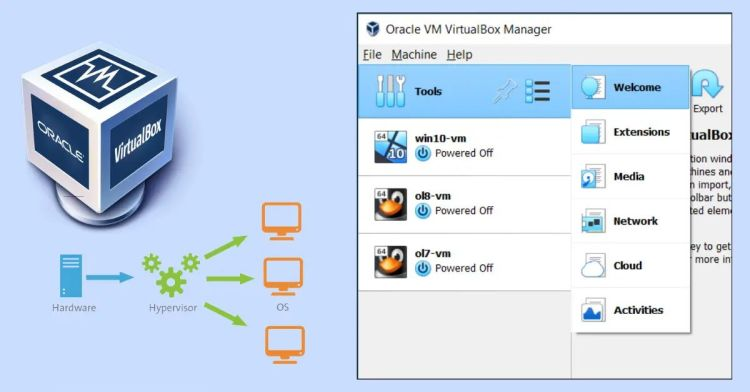
\includegraphics[width=1.0\textwidth]{Oracle_cloud/virtualbox.jpg}
    \caption{Oracle VM VirtualBox}
    \label{fig:cloud_intro}
\end{figure}

\subsubsection{Đặc điểm của Oracle VM Server}
Oracle VM Server không chỉ đáp ứng đầy đủ các chức năng cơ bản của một nền tảng ảo hóa, mà còn sở hữu những tính năng nâng cao, giúp nó trở thành một trong những giải pháp mạnh mẽ và khác biệt trên thị trường.

\begin{myitem}

\item Tính sẵn sàng cao (High Availability – HA)

\hspace*{1cm} Oracle VM Server được thiết kế với cơ chế tự động khởi động lại các máy ảo bị lỗi trên các máy chủ khác trong cùng Server Pool. Khi một máy chủ gặp sự cố, các máy ảo đang chạy trên đó sẽ được chuyển sang máy chủ khác một cách tự động, giúp giảm thiểu thời gian chết và đảm bảo dịch vụ vẫn hoạt động liên tục.

\hspace*{1cm} Điều này đặc biệt quan trọng trong môi trường trung tâm dữ liệu hoặc các ứng dụng doanh nghiệp yêu cầu tính liên tục cao, nơi bất kỳ gián đoạn nào cũng có thể ảnh hưởng đến hoạt động kinh doanh hoặc gây mất dữ liệu quan trọng. Nhờ tính năng HA, Oracle VM Server giúp doanh nghiệp yên tâm vận hành các ứng dụng quan trọng mà không lo gián đoạn.

\item Khả năng mở rộng và hiệu suất mạnh mẽ

\hspace*{1cm} Oracle VM Server dựa trên kiến trúc Xen Hypervisor tối ưu, giúp đạt hiệu suất cao nhưng vẫn giữ chi phí hợp lý. Nó có khả năng hỗ trợ lên tới 384 CPU vật lý và 6TB RAM, đáp ứng nhu cầu xử lý khối lượng công việc lớn trong môi trường đám mây và doanh nghiệp.

\hspace*{1cm} Đối với mỗi máy ảo, người dùng có thể cấu hình tới 256 CPU ảo và 2TB RAM. Với cấu hình này, Oracle VM Server có thể chạy mượt các ứng dụng phức tạp như ERP, CRM hoặc các hệ thống phân tích dữ liệu lớn (Big Data). Điều này giúp doanh nghiệp triển khai các dịch vụ nặng mà không lo thiếu tài nguyên, đồng thời tối ưu hóa hiệu quả vận hành.

\item Quản lý tập trung và nâng cao mà không tốn thêm chi phí

\hspace*{1cm} Oracle VM Server đi kèm với Oracle VM Manager, cung cấp giao diện quản lý tập trung dựa trên trình duyệt web. Người quản trị có thể dễ dàng quản lý các tài nguyên như máy ảo, nhóm máy chủ, lưu trữ và mạng, đồng thời theo dõi sự kiện và tình trạng hệ thống theo thời gian thực.

\hspace*{1cm} Nhờ tính năng quản lý tập trung này, doanh nghiệp không cần đầu tư thêm các công cụ quản lý bên ngoài. Việc phân bổ và giám sát tài nguyên trở nên hiệu quả hơn, giúp tiết kiệm chi phí vận hành và tránh phụ thuộc vào phần mềm thứ ba. Điều này đặc biệt hữu ích với các doanh nghiệp muốn duy trì hiệu quả vận hành mà vẫn kiểm soát chi phí.

\item Hỗ trợ đa dạng hệ điều hành

\hspace*{1cm} Oracle VM Server có thể chạy nhiều hệ điều hành khác nhau, bao gồm Oracle Linux, Oracle Solaris, Enterprise Linux, SUSE Linux Enterprise, Red Hat Enterprise Linux (RHEL), CentOS và các phiên bản phổ biến của Microsoft Windows.

\hspace*{1cm} Khả năng này giúp doanh nghiệp triển khai hạ tầng đa nền tảng mà vẫn đồng bộ trong cùng một hệ thống ảo hóa. Nhờ đó, các ứng dụng trên nhiều hệ điều hành khác nhau có thể cùng vận hành hiệu quả, nâng cao tính linh hoạt và khả năng tương thích của hạ tầng công nghệ thông tin.

\item Chuyển đổi máy ảo an toàn (Secure Live VM Migration)

\hspace*{1cm}Oracle VM Server hỗ trợ di chuyển trực tiếp các máy ảo đang chạy (live migration) từ máy chủ này sang máy chủ khác mà không gây gián đoạn dịch vụ. Quá trình di chuyển được thực hiện thông qua SSL URL an toàn, bảo vệ dữ liệu và kết nối trong suốt quá trình.

\hspace*{1cm} Tính năng này rất hữu ích khi doanh nghiệp cần bảo trì hệ thống theo kế hoạch hoặc mở rộng, tái phân bổ tài nguyên. Nhờ đó, dịch vụ luôn hoạt động liên tục, người dùng cuối không bị gián đoạn, giúp tăng tính ổn định và độ tin cậy của toàn bộ hệ thống.
\end{myitem}

\subsubsection{Ưu điểm – hạn chế của Oracle VM Server}
\begin{myitem}
\item Ưu điểm.

  \begin{mysubitem}
    \item Oracle VM hỗ trợ đa dạng nền tảng, tương thích với cả máy chủ x86 lẫn hệ điều hành Solaris. Ngoài ra, công cụ này còn cho phép nhân bản máy ảo (VM cloning), giúp triển khai nhanh chóng các hệ thống mới mà không cần cấu hình từ đầu, tiết kiệm đáng kể thời gian và công sức cho các quản trị viên.
    
    \item Về khả năng quản lý, Oracle VM cung cấp Oracle VM Manager với cả giao diện dòng lệnh (CLI) và Web Services API (WS-API). Điều này cho phép mức độ tự động hóa cao, giúp dễ dàng tích hợp Oracle VM với các hệ thống quản lý công nghệ thông tin khác, từ đó tối ưu hóa việc giám sát và vận hành hạ tầng ảo.
    
    \item Quá trình cài đặt và cấu hình Oracle VM cũng khá đơn giản, không đòi hỏi nhiều bước phức tạp. Điều này giúp việc triển khai nhanh chóng và đưa vào vận hành ngay, phù hợp với môi trường doanh nghiệp cần triển khai các dịch vụ mới một cách kịp thời.
    
    \item Oracle VM còn nổi bật về khả năng mở rộng và hiệu suất. Một máy chủ vật lý có thể chạy tối đa 128 máy ảo, đáp ứng tốt nhu cầu của các trung tâm dữ liệu lớn hoặc môi trường điện toán đám mây. Nhờ tận dụng kiến trúc Xen Hypervisor tối ưu, hiệu năng của các máy ảo cũng rất ổn định, giảm thiểu tình trạng nghẽn hay gián đoạn trong vận hành.
    
    \item Oracle VM Templates hỗ trợ triển khai các ứng dụng doanh nghiệp phức tạp như ERP, CRM hay cơ sở dữ liệu Oracle chỉ trong vài bước đơn giản, rút ngắn đáng kể thời gian cài đặt và cấu hình. Thêm vào đó, Oracle còn cung cấp máy ảo miễn phí phục vụ thử nghiệm, nghiên cứu và phát triển, hỗ trợ tốt cho các nhà phát triển và quản trị viên hệ thống muốn tìm hiểu hoặc triển khai thử nghiệm mà không tốn chi phí.

  \end{mysubitem}

\item Hạn chế

  \begin{mysubitem}
    \item Phụ thuộc nhiều vào hệ sinh thái Oracle. Nếu hạ tầng công nghệ thông tin chủ yếu dựa trên các công nghệ không thuộc Oracle, việc tích hợp có thể gặp khó khăn, gây cản trở cho các doanh nghiệp có môi trường đa nền tảng.
    
    \item Việc thiết lập và quản lý tường lửa trên Oracle VM đôi khi khá phức tạp, đặc biệt trong môi trường doanh nghiệp với nhiều lớp bảo mật. Điều này đòi hỏi quản trị viên phải có kiến thức chuyên sâu và dành thời gian nhiều hơn để cấu hình an toàn.
    
    \item Mặc dù Oracle VM Templates giúp triển khai nhanh, nhưng các mẫu có sẵn vẫn chưa đa dạng, đặc biệt với các Oracle Database nodes. Người dùng thường phải tự cấu hình nhiều hơn, gây mất thời gian và tăng nguy cơ lỗi nếu không am hiểu kỹ thuật.
    
    \item Giao diện quản lý người dùng (UI) của Oracle VM Manager cũng được đánh giá khó sử dụng hơn so với các đối thủ như VMware vSphere. Người dùng cần có kiến thức chuyên sâu để khai thác đầy đủ các tính năng, khiến việc vận hành ban đầu trở nên phức tạp.
    
    \item Việc xây dựng Private Cloud và triển khai các tính năng tự động hóa đám mây trên Oracle VM vẫn còn gặp nhiều khó khăn. Quá trình này đòi hỏi nhiều công tác bảo trì, nâng cấp và quản lý, dẫn đến tốn kém thời gian và nhân lực nếu doanh nghiệp muốn tận dụng tối đa các tính năng đám mây riêng.
  \end{mysubitem}

\end{myitem}

\newpage
\subsection*{\centering KẾT LUẬN CHƯƠNG 2}
\addcontentsline{toc}{subsection}{KẾT LUẬN CHƯƠNG 2}

Chương 2 đã trình bày tổng quan về công nghệ ảo hóa trong Oracle Cloud, bao gồm các khái niệm cơ bản, kiến trúc ảo hóa, các loại máy chủ ảo trong Oracle VM và các tính năng nổi bật của Oracle VM Server. Qua đó, có thể nhận thấy ảo hóa là nền tảng quan trọng giúp tối ưu hóa sử dụng tài nguyên phần cứng, nâng cao hiệu suất vận hành, tăng khả năng mở rộng và cải thiện tính bảo mật cho hệ thống doanh nghiệp.

Oracle VM Server, với sự tích hợp Xen Hypervisor và Oracle VM Manager, cung cấp một giải pháp ảo hóa mạnh mẽ, hỗ trợ đa dạng hệ điều hành, quản lý tập trung, chuyển đổi máy ảo an toàn và tính sẵn sàng cao. Những ưu điểm này giúp doanh nghiệp triển khai các ứng dụng và dịch vụ quan trọng một cách hiệu quả, giảm thiểu gián đoạn và tối ưu chi phí vận hành.

Bên cạnh đó, chương cũng chỉ ra những hạn chế như phụ thuộc vào hệ sinh thái Oracle, một số tính năng quản lý và UI phức tạp, cũng như hạn chế về đa dạng mẫu máy ảo. Nhìn chung, Oracle VM Server vẫn là một giải pháp ảo hóa đáng tin cậy, phù hợp với môi trường doanh nghiệp và trung tâm dữ liệu, đồng thời đóng vai trò nền tảng cho triển khai các dịch vụ đám mây và mô hình IT as a Service.
